\documentclass[11pt]{article}
\usepackage[margin=1.5cm]{geometry}
\usepackage{amsmath, amssymb, graphicx}
\usepackage{lscape}

\begin{document}
\title{ChemTreeN Analysis Notes}
\author{C.Coleman-Smith\\ cec24@phy.duke.edu}
\date{\today}
\maketitle

\section{introduction}

The chem tree N code is a galaxy formation simulation. The code simulates the evolution of clusters of dark matter through a spatially tree'd n-body simulation, mergings of the dark matter lead to the formation of clusters and eventually galaxies. A run of this gravitational code produces a dark matter merger tree, describing the evolution of the initial Gaussian field of matter into a  clustered and bound galaxy with outliers. A single merger tree is then used to explore the variation of the underlying ``chemical'' (actually nuclear) processes which determine stellar formation and evolution. This secondary evolution is described by a set of coupled ODE's, it is entirely relatively deterministic. The evolution of the dark matter itself, is likely to be somewhat statistical in nature owing to the approximations underlying any practical n-body code. 

It is a important to know which values of the parameters determining the secondary (or deterministic) evolution of the simulation into its final state produce configurations similar to those that have been observed both in our own galaxy \footnote{which may be quite a remarkable galaxy} and in others. 

In this study we have identified two observables which can be profitably explored: the metallicity in star clusters and the cumulative luminosity. The metallicity referrers to the relative fraction of material in a star which is heavier than He (H?). The cumulative luminosity is a cumulative measure of the number of satellite galaxies which have luminosity greater than a certain magnitude. (need to explain magnitudes here?)

For a preliminary run field observations of the luminosity at 4 magnitudes and the metallicity were created from a ``prior best'' model configuration. 

In this note i will outline the design and analysis of the first wave of this code. We emulate the output of the various observations of the model, compute a measure of how feasible the output is at various locations in the parameter space. Finally I outline how to select a region in which all of the observables under scrutiny are within some acceptable distance from their measured values, this final ``good volume'' then needs to be further investigated by a creating a new design. 

The creation of a new design in the favored volume will be treated in a subsequent note.

\section{Design}

Three parameters from the deterministic evolution were selected to be varied.
\begin{itemize}
\item The halo formation stop time $Z_r$, this is a red-shift in the range $[20, 5]$ with a typical value of $10$.
\item The fraction of metal escaping from a dying star $F_{escp}$. This is a percent in the range $[0,100]$ with a typical value of $50$.
\item The fraction of baryons initially in a galaxy $F_{bary}$. This is a percent which should be in the range $[0, 0.2]$, a typical value is $0.05$.
\end{itemize}

A Latin Hyper-cube design with $45$ points was created to span the space $\{Z_r, F_{escp}, F_{bary}\}$, runs were carried out at MSU by F.Gomez.

\section{luminosity}

The luminosity spectrum (see Fig:~\ref{fig-lum-typical}) is typically reported as the cumulative distribution of the number of satellite galaxies with magnitude below a given value. Instead of dealing with the spectrum as a continuous object we sampled the spectrum at the follow representative values $M_{sample} = \{ -15.5, -11.5, -7.5, -3.5\}$. Recall that magnitude is a reversed log scale, more positive numbers are brighter. 

\begin{figure}
  \begin{center}
    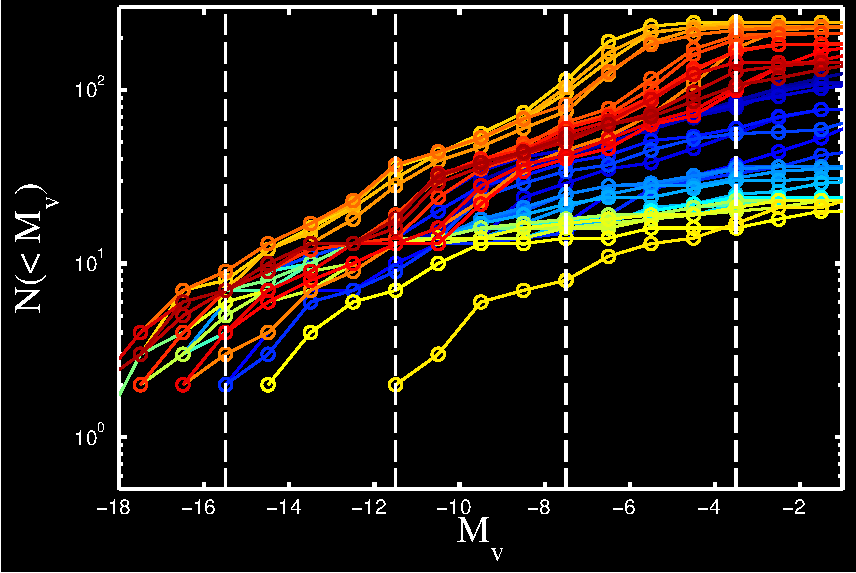
\includegraphics[width=0.5\textwidth]{./images/lf.pdf}
    \caption{A typical cumulative luminosity spectrum, the dashed lines indicate the luminosity's at which we have analyzed the model}
    \label{fig-lum-typical}
  \end{center}
\end{figure}

\begin{table}
  \begin{center}
    \begin{tabular}{l c c c r}
      M & -15.5 & -11.5 & -7.5 & -3.5 \\
      \hline
      L & 5 & 13 & 41 & 83 \\
      $\sigma$ & 2.23 & 3.605 & 6.4 & 9.11
    \end{tabular}
    \caption{ The observed values of the luminosity $L$ for the 4 magnitude bins $M$ with associated standard errors $\sigma$}
    \label{tab-lum-obs}
  \end{center}
\end{table}


The model results for each luminosity bin are shown in Fig:~\ref{fig-lum-vs-exp}, the field observations are shown with a $90\%$ confidence interval (see Table:~\ref{tab-lum-obs}). The brightest bin seems to have generally been less well reproduced than the others. Each point in the design set produces a value of the luminosity at each of the four locations, the results for each bin are therefore not independent. There are methods for dealing with dependent scalar observations  (cite kernel paper). We shall begin by making independent emulators for each of the bins and then enforcing requirements of ``goodness'' across all four outputs at a given point (as in the galform paper). The spread in the model results over the luminosity bins increases rapidly.

Projecting the model output against each dimension in turn reveals some underlying structure Fig:~\ref{fig-lum-vs-design}, especially in the $Z_r$ dimension of the brighter bins. 

\begin{figure}
  \begin{center}
    \includegraphics[width=0.5\textwidth]{./images-lum/lum-exp-vs-model.pdf}
    \caption{Observed luminosity (black q's with error bars) against modeled luminosity. Each of the 45 model runs produces an output at all 4 luminosity bins. The performance of the model at the various design locations becomes more variable with increasing luminosity, the final luminosity bin is rather badly represented.}
    \label{fig-lum-vs-exp}
  \end{center}
\end{figure}

\begin{landscape}
  \begin{figure}
    \begin{center}
      \includegraphics[width=\textwidth]{./images-lum/lum-all-vs-design.pdf}
      \caption{The variation of the model output for each luminosity bin is projected against each dimension in the design. }
      \label{fig-lum-vs-design}
    \end{center}
  \end{figure}
\end{landscape}

We trained an emulator with a power-exponential co-variance function and a first order regression model on the model data. The hyper parameters, which determine the characteristic length scales, were estimated numerically by a maximum likelihood method. The scalar likelihood, which is a 5 dimensional object, can be projected onto pairs of the hyper-parameters Fig:~\ref{fig-lhood-contours}. 

\begin{figure}
  \begin{center}
    \includegraphics[width=0.8\textwidth]{./images-lum/lhood-compare-bin-1.pdf}
    \caption{The likelihood distribution for the first luminosity bin projected onto orthogonal sections. The cross marks the location obtained from the numerical maximization routines.} 
    \label{fig-lhood-contours}
  \end{center}
\end{figure}

The following table lists the values estimated for the hyper-parameters for each observed bin
\begin{table}
\begin{center}
\begin{tabular}{l c c c c r}
Magnitude & Scale & Nugget & $\theta_{Zr}$ & $\theta_{Fescp}$ & $\theta_{Fbary}$ \\
\hline
-15.5 & 1e-05 & 0.004330937 & 0.1350121 &  3.071656 & 0.8854663 \\
-11.5 & 1e-05 & 0.000010000 & 0.2407256 & 46.457078 & 0.5644926  \\
-7.5 & 1e-05 & 0.000010000 & 0.1332110 & 13.362850 & 1.3600413 \\
-3.5 & 1e-05 & 0.000010000 & 0.2442450 &  1.659991 & 4.15787181 \\
\end{tabular}
\caption{Estimated hyper parameters for separate emulators trained on the observed luminosity at different magnitudes.}
\label{tab-theta-values-lum}
\end{center}
\end{table}

It is apparent in Table:~\ref{tab-theta-values-lum} that the length scales in the $F_{escp}$ dimension are very long, this is also clear in Fig:~\ref{fig-lum-vs-design}. This suggests that this parameter is not strongly influential on the observed luminosity.
 We can verify the estimated thetas by doing a round-robin (k-withhold) test, here the design is partitioned into $k$ subsets. The emulator is then successively trained on the complements of each subset, predictions from the emulator are obtained for the value at these withheld points. These predictions can then be compared against the value already obtained from the model and we can build up some degree of confidence in the emulator, typically we compare the predictions $\hat{y}_{\mbox{emu}}$  as
\begin{equation}
\label{eqn-z-deviates}
Z = \sum_{i\in\mbox{withheld}}\frac{\left(E[{y}(x_{i})] - y_{\mbox{true}}(x_{i}) \right)^2 }{V[y(x_i)]}.
\end{equation}

A crude measure of the performance of the emulator is to compute the fraction of points with  $Z > 2$ this gives a rough idea of how many points are relatively well emulated, with $Z < 2$ and how many are currently poorly treated. For the current design this ratio is shown in Table:~\ref{tab-z-ratios-lum}, these results suggest that we currently do not have a large enough design to get a really good treatment of the model across the space. Repeating the experiment with a larger design would be advisable before launching into the iterative descent process.

\begin{table}
\begin{center}
\begin{tabular}{l c c c r}
M & -15.5 & -11.5 & -7.5 & -3.5 \\
\hline
$Z_r$ & 0.28 & 0.09 & 0.31 & 0.24 \\
\end{tabular}
\caption{Fraction of model points poorly treated by the best possible emulator}
\label{tab-z-ratios-lum}
\end{center}
\end{table}

\begin{figure}
  \begin{tabular}{l c r}
    \includegraphics[width=0.3\textwidth]{./images-lum/hold-back-Zr.pdf}  &
    \includegraphics[width=0.3\textwidth]{./images-lum/hold-back-Fescp.pdf}  & 
    \includegraphics[width=0.3\textwidth]{./images-lum/hold-back-Fbary.pdf}
  \end{tabular}
  \caption{Showing the deviation of the predicted value from the known model value across the design space.}
  \label{fig-deviates-lum-fun}
\end{figure}

It is still interesting to make some predictions with our emulator across the design space, although we should not be very confident in the resulting predictions. In Fig~\ref{fig-emulator-slices} we show slices through the $\{Z_r, F_{escp}, F_{bary}\}$ space by plotting the $\{Z_r, F_{bary}\}$ plane at successive values of $F_{escp}$. Since the $F_{escp}$ dimension is the most slowly varying it is reasonable to project onto the two ``fast'' dimensions. 

\begin{figure}
  \begin{tabular}{l r} 
    \includegraphics[width=0.5\textwidth]{./images-lum/emu-mean-stepped-lum-bin-1-cov-1.pdf} &
    \includegraphics[width=0.5\textwidth]{./images-lum/emu-mean-stepped-lum-bin-2-cov-1.pdf} \\
    \includegraphics[width=0.5\textwidth]{./images-lum/emu-mean-stepped-lum-bin-3-cov-1.pdf} &
    \includegraphics[width=0.5\textwidth]{./images-lum/emu-mean-stepped-lum-bin-4-cov-1.pdf} \\
  \end{tabular}
  \caption{The emulated mean for each luminosity bin projected $-15.5, -11.5, -7.5, -3.5$ (left to right) into slices in the $\{Z_r, F_{bary}\}$ plane. The scattered points represent the design locations as projected into the plane. Little variation is observed in the stepped direction. The observed values for each bin are $5, 13, 41, 83$.}
  \label{fig-emulator-slices}
\end{figure}


We can compute a measure of the deviation of the value of the luminosity as predicted by our model and the emulator against the observed field values as given in Table:\ref{tab-lum-obs}, this value is referred to as an implausibility measure in the galform paper
\[
I = \frac{ ( E[y(x_{i})] - y_{obs})^2 }{Var[y(x_{i})] + Var[y_{obs}]}.
\] 

This is computed for each luminosity bin and slices through the
$\{Z_{r}, F_{bary} \}$ plane are shown in
Fig~\ref{fig-implaus-slices}. We can simply combine the various
observation bins  by constraining their maximum value at each point in
the design space, see Fig:~\ref{fig-implaus-comb-slices}. The
combined luminosity data shows a slightly sloped slab extending
vertically in the $F_{escp}$ dimension. This feasible slice should
contain the real training parameters used to generate the field
data. 

To move forwards we can repeat the analysis with the metallicity
output and then simply combine the implausibility of all
observables. After this we need to consider how to go about creating a
refined design and how to address the issues of the poor emulator
performance in the current design. 


\begin{figure}
  \begin{center}
    \large{Luminosity Implausibility}
  \end{center}
  \begin{tabular}{l r} 
    \includegraphics[width=0.5\textwidth]{./images-lum/implaus-stepped-lum-bin-1-cov-1.pdf} &
    \includegraphics[width=0.5\textwidth]{./images-lum/implaus-stepped-lum-bin-2-cov-1.pdf} \\
    \includegraphics[width=0.5\textwidth]{./images-lum/implaus-stepped-lum-bin-3-cov-1.pdf} &
    \includegraphics[width=0.5\textwidth]{./images-lum/implaus-stepped-lum-bin-4-cov-1.pdf} \\
  \end{tabular}
  \caption{The implausibility for each luminosity bin projected $-15.5,
    -11.5, -7.5, -3.5$ (left to right) into slices in the $\{Z_r,
    F_{bary}\}$ plane. Hotter values are more plausible, the threshold
    value is plotted as solid red.}
  \label{fig-implaus-slices}
\end{figure}


\begin{figure}
  \begin{center}
    \includegraphics[width=\textwidth]{./images-lum/implaus-stepped-comb-cov-1.pdf}
    \caption{Max Implausibility at each point evaluated by comparing
      all luminosity bins. The data is cut on $I_{max} <
      1.8$, there is a clear ``acceptable'' slice through the
      space.}
    \label{fig-implaus-comb-slices}
    \end{center}
\end{figure}

\begin{figure}
  \begin{center}
    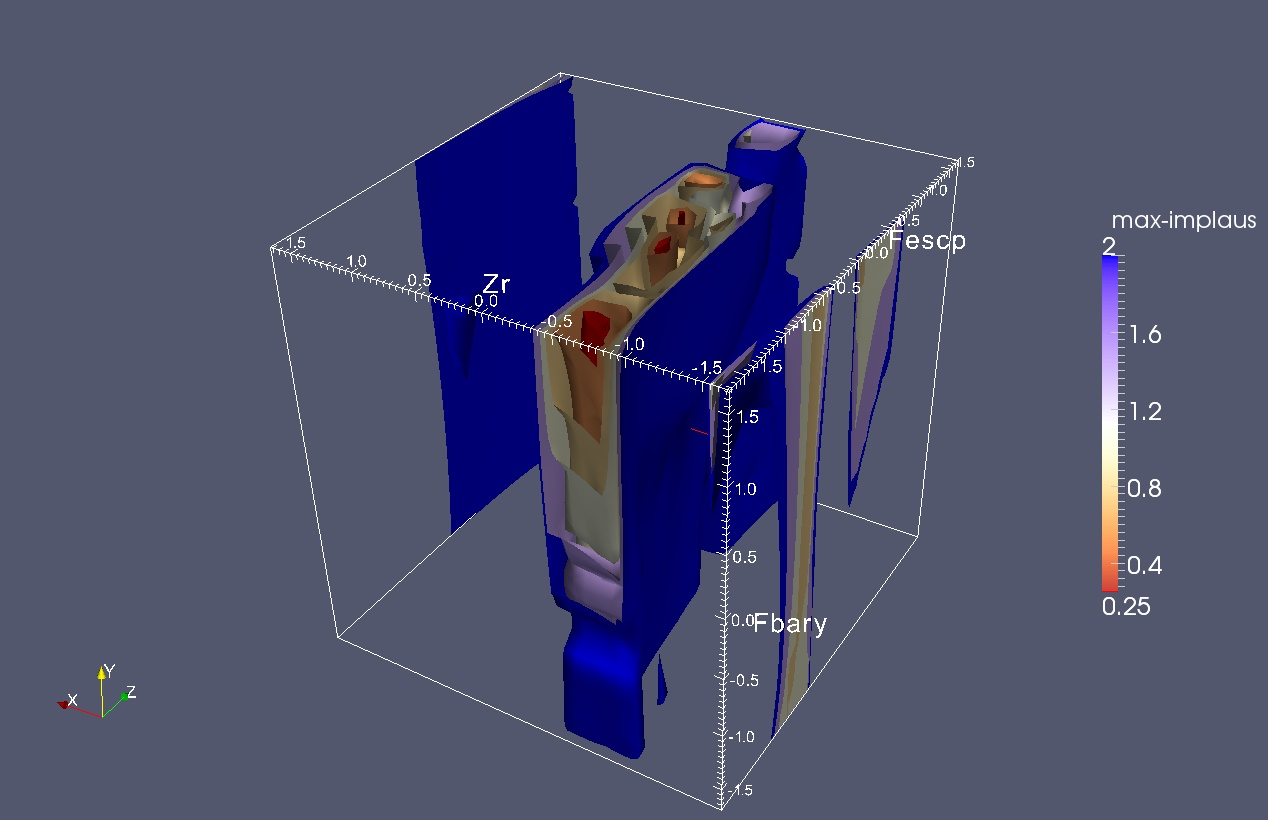
\includegraphics[width=\textwidth]{./images/lum-anim.jpg}
    \caption{Max Implausibility at each point evaluated by comparing
      all luminosity bins. \emph{In 3d!} The design is presented
      scaled and centered. This is not a desired feature. The implausibility
      is cut on $I_{max} < 2$ with contours drawn at $\{0.25, 0.5, 0.75,
      1.0, 1.5, 2.0\}$.}
    \label{fig-implaus-comb-cube}
    \end{center}
\end{figure}


\section{metallicity}

The metallicity data are the two components (slope $a11$ and intercept
$a21$) nof a linear fit to the
actual metallicity spectrum. We repeat the above process for this
data. The observed data are given as the values of the coefficients
plus a $95\%$ confidence interval, see Table~\ref{tab-met-obs}. Since
the observed values are rather separated  a direct visual comparison
is not very instructive. 

Fig:~\ref{fig-met-vs-run} shows the variation of the two coefficients
over the design in terms of the run number. Each the position in
design space is relatively random a LHS design is typically somewhat
sequentially space filling. As such the variation seen in this figure
suggests that there is some actual variation across this design space,
as seen in Fig:~\ref{fig-met-all-vs-design}. The computed coefficients exhibit
a relatively smooth spatial variation in the $\{Z_R,
F_{escp}\}$ plane. Recall that this was found to be the more important
direction for the luminosity data computed on the same design. The
apparent ``smoothness'' of these trends contrasts with the luminosity data.

\begin{table}
  \begin{center}
    \begin{tabular}{l c r}
      \ & slope & intercept \\
      \hline
      coeff & -0.061 & -2.402 \\
      conf & 0.0039 & 0.0258 
    \end{tabular}
    \caption{ The observed values of the luminosity $L$ for the 4 magnitude bins $M$ with associated standard errors $\sigma$}
    \label{tab-met-obs}
  \end{center}
\end{table}

\begin{figure}
\begin{center}
  \large{Metallicity model output}
  \includegraphics[width=\textwidth]{./images-met/met-all-vs-run.pdf}
  \caption{ Contrasting the ``experimentally'' observed metallicity coefficients (black
    crosses with \emph{error} bars), against the model output (red
    crosses) as a function of the model run index }
  \label{fig-met-vs-run}
  \end{center}
\end{figure}

\begin{figure}
  \begin{center}
    \includegraphics[width=\textwidth]{./images-met/met-all-vs-design.pdf}
    \caption{ The model output projected across the design space (crosses)
      compared with the experimentaly observed values (blue lines with
      $95\%$ confidence bands).  More significant spatial variation in the $\{Z_R,
      F_{escp}\}$ plane is observed
      compared to the luminosity  data Fig:~\ref{fig-lum-vs-design}.}
    \label{fig-met-all-vs-design}
  \end{center}
\end{figure}

We proceed to train an emulator on this data set and list the
resulting length scales in Table:~\ref{tab-theta-values-met}. We
list the performance of this emulator interms of the fraction of
poorly treated points derived by a $k$ withhold test, we find
relatively good performance with 
\begin{align*}
Z_{a11} &= 0.022 \\
Z_{a21} &= 0.089,
\end{align*}
the model values for both coefficients can be reproduced with less
than $10\%$ of the model points being badly treated. This is
remarkably better performance is doubtless due to the greater degree
of variation of the data across the design space. Emulators perform
fairly poorly on very slowly changing (or stationary) data with a
small number of sharp jumps as is the case with the current luminosity
data set.

\begin{table}
  \begin{center}
    \begin{tabular}{l c c c c r}
      coeff & Scale & Nugget & $\theta_{Zr}$ & $\theta_{Fescp}$ & $\theta_{Fbary}$ \\
      \hline
      a11 & 1.322 & 0.002 & 8.055 & 0.416 & 0.415 \\
      a21 & 1.371 & 0.005 & 0.356 & 0.209 & 5.971
    \end{tabular}
    \caption{Estimated hyper parameters for separate emulators trained on
      the modelled metallicity fit coefficients.}
    \label{tab-theta-values-met}
  \end{center}
\end{table}


The deviations shown in Fig:~\ref{fig-deviates-met} show again that
most of the model points are well treated by this design \& emulator.

\begin{figure}
    \begin{center}
      \large{Metallicity Emulator deviation}
    \end{center}
  \begin{tabular}{l c r}
    \includegraphics[width=0.3\textwidth]{./images-met/hold-back-Zr.pdf}  &
    \includegraphics[width=0.3\textwidth]{./images-met/hold-back-Fescp.pdf}  & 
    \includegraphics[width=0.3\textwidth]{./images-met/hold-back-Fbary.pdf}
  \end{tabular}
  n  \caption{Showing the deviation of the predicted value from the known model value across the design space.}
  \label{fig-deviates-met}
\end{figure}

The predicted value of each of the cofficients varied across the
design space by projecting into the $\{Z_r, F_{escp}\}$ plane and
stepping in the $F_{bary}$ direction are shown in
Fig:~\ref{fig-emulator-slices-met}.

\begin{figure}
  \begin{center}
    \large{Emulated Metallicity}
  \end{center}
    \includegraphics[width=0.5\textwidth]{./images-met/emu-mean-stepped-met-bin-1.pdf} 
    \includegraphics[width=0.5\textwidth]{./images-met/emu-mean-stepped-met-bin-2.pdf} \\
  \caption{The emulated mean for each metallicity coefficient projected into
    slices in the $\{Z_r, F_{bary}\}$ plane. The scattered points
    represent the design locations as projected into the plane. Less
    variation is observed in the stepped direction. The observed
    values are $-0.061 \pm 0.0039, -2.402 \pm 0.0258$.}
  \label{fig-emulator-slices-met}
\end{figure}


Finally we present the implausibility for each coefficient in Fig:~\ref{fig-implaus-slices-met} and the combined maximum implausibility (over metallicity coefficients) in Fig:~\ref{fig-implaus-comb-slices-met}.


\begin{figure}
  \begin{center}
    \large{Metallicity Implausibility}
  \end{center}
    \includegraphics[width=0.5\textwidth]{./images-met/implaus-stepped-met-bin-1.pdf} 
    \includegraphics[width=0.5\textwidth]{./images-met/implaus-stepped-met-bin-2.pdf} \\
  \caption{The implausibility for each metallicity coefficient projected into slices in the $\{Z_r,
    F_{bary}\}$ plane. Hotter values are more plausible, the threshold
    value is plotted as solid red. Given the current errors on the data it is clear that there is a huge accceptable region spanning most of the design}
  \label{fig-implaus-slices-met}
\end{figure}


\begin{figure}
  \begin{center}
    \includegraphics[width=\textwidth]{./images-met/implaus-stepped-comb.pdf}
    \caption{Max Implausibility at each point evaluated by comparing
      both metallicity coefficients. The data is cut on $I_{max} <
      1.8$. There is a large \emph{very good} ($I < 0.2$) region amorphously in the center of the design. Even the worst values are not very bad in this case  }
    \label{fig-implaus-comb-slices-met}
    \end{center}
\end{figure}



\end{document}
